\section{Preliminary design}
	Based on the selected concept the simplest body diagram has been created in order to start the dimensioning of the main elements of the structure. Considering the possible practical implementation of the system, the symbolic representation of the moving frame has been made (figure \ref{fig:freebodydiagramframe}).
	
	\begin{figure}[bht]
		\centering 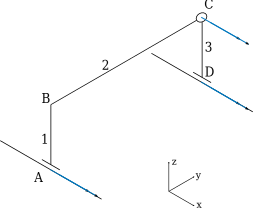
\includegraphics{preliminary-a}
		\caption{schematic representation of the moving frame supporting the arm; blue arrows are describes the rotational degree of freedom left by the joints.}
		\label{fig:freebodydiagramframe}
	\end{figure}
	
	The design involves a main elevated track (body 2) supported by two vertical supporting beams (bodies 1 and 3); the connection between body 1 and 2 is constituted by a full joint in point $B$ constraining all 6 degrees of freedom while the connection of the track with the other support is done by a hinge that leaves free the rotation over the global $x$ axis. The two vertical supports can slide on two parallel tracks and the associated prismatic joints constraints respectively 5 and 4 degrees of freedom in $A$ and $D$, leaving the system free to slide along the $x$ global axis; the choice of leaving also $D$ in as free to rotate aims at reducing redundant constraints, reducing hyperstatic variables with a design that accommodates misalignments in the position of the two parallel tracks placed at ground.
	
	
	\begin{figure}[p]
		\begin{subfigure}{\linewidth}			
			\centering 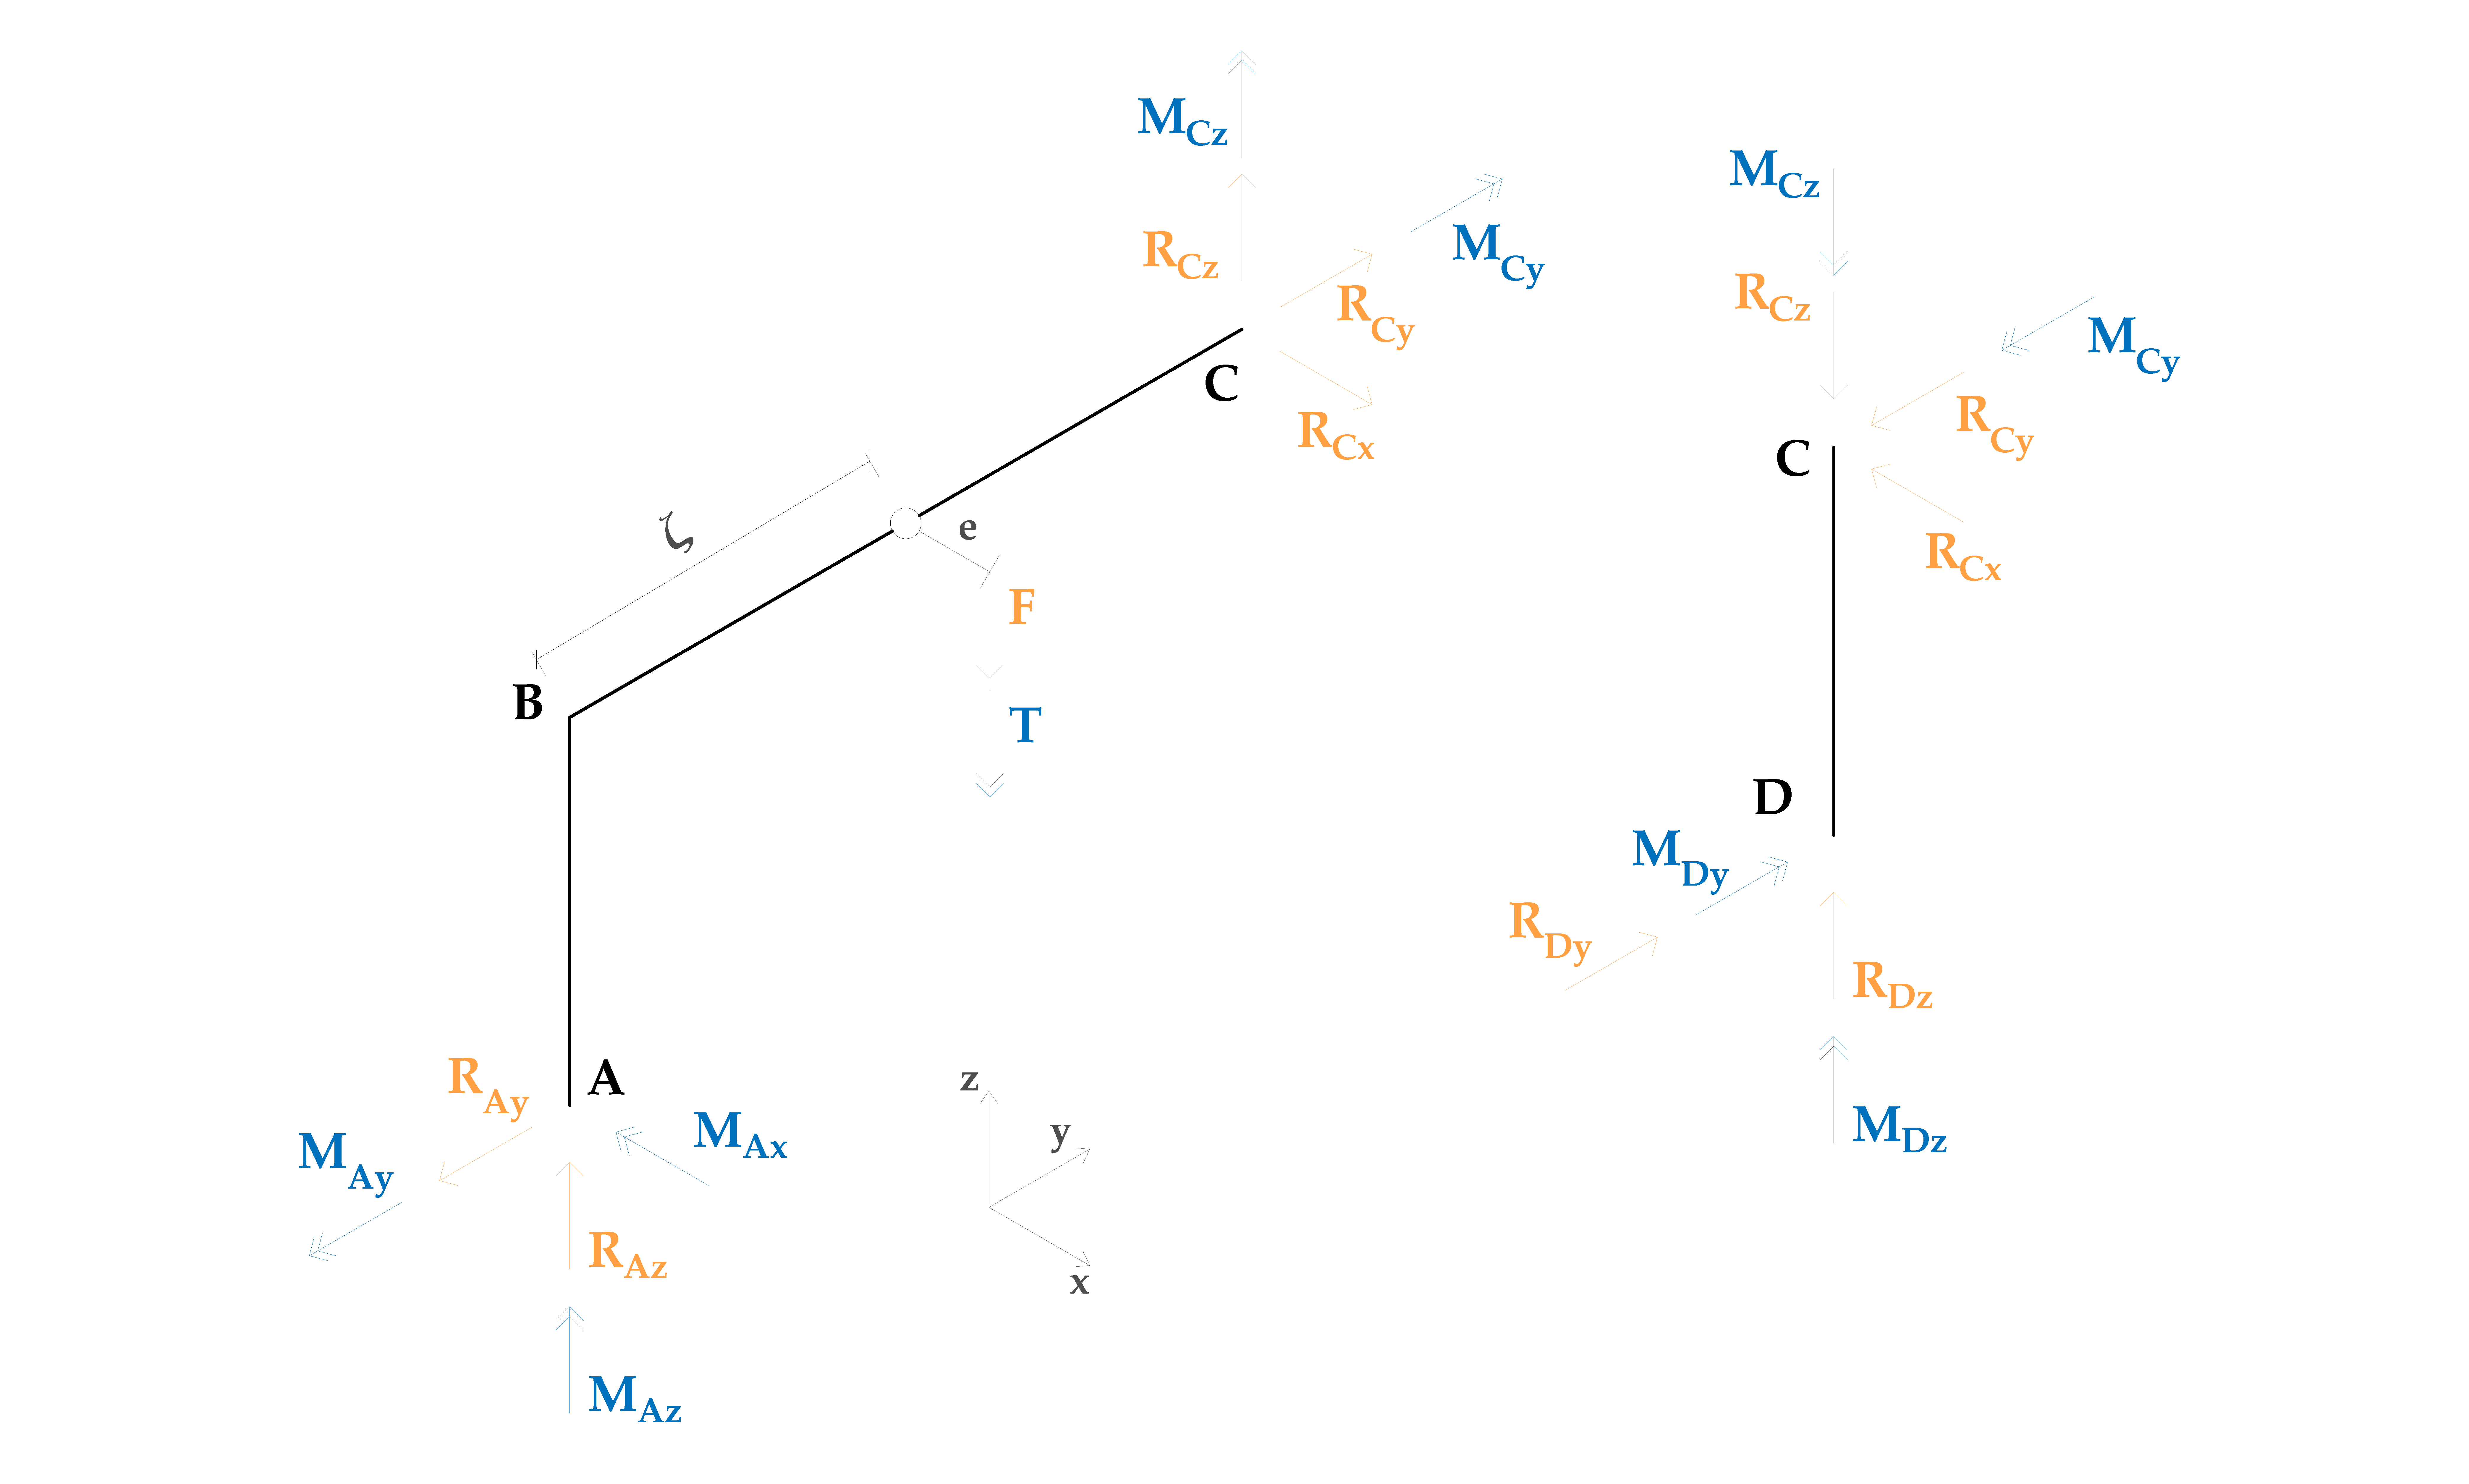
\includegraphics[width=15cm]{reactions} \caption{}
		\end{subfigure}
		\begin{subfigure}{\linewidth}			
			\centering 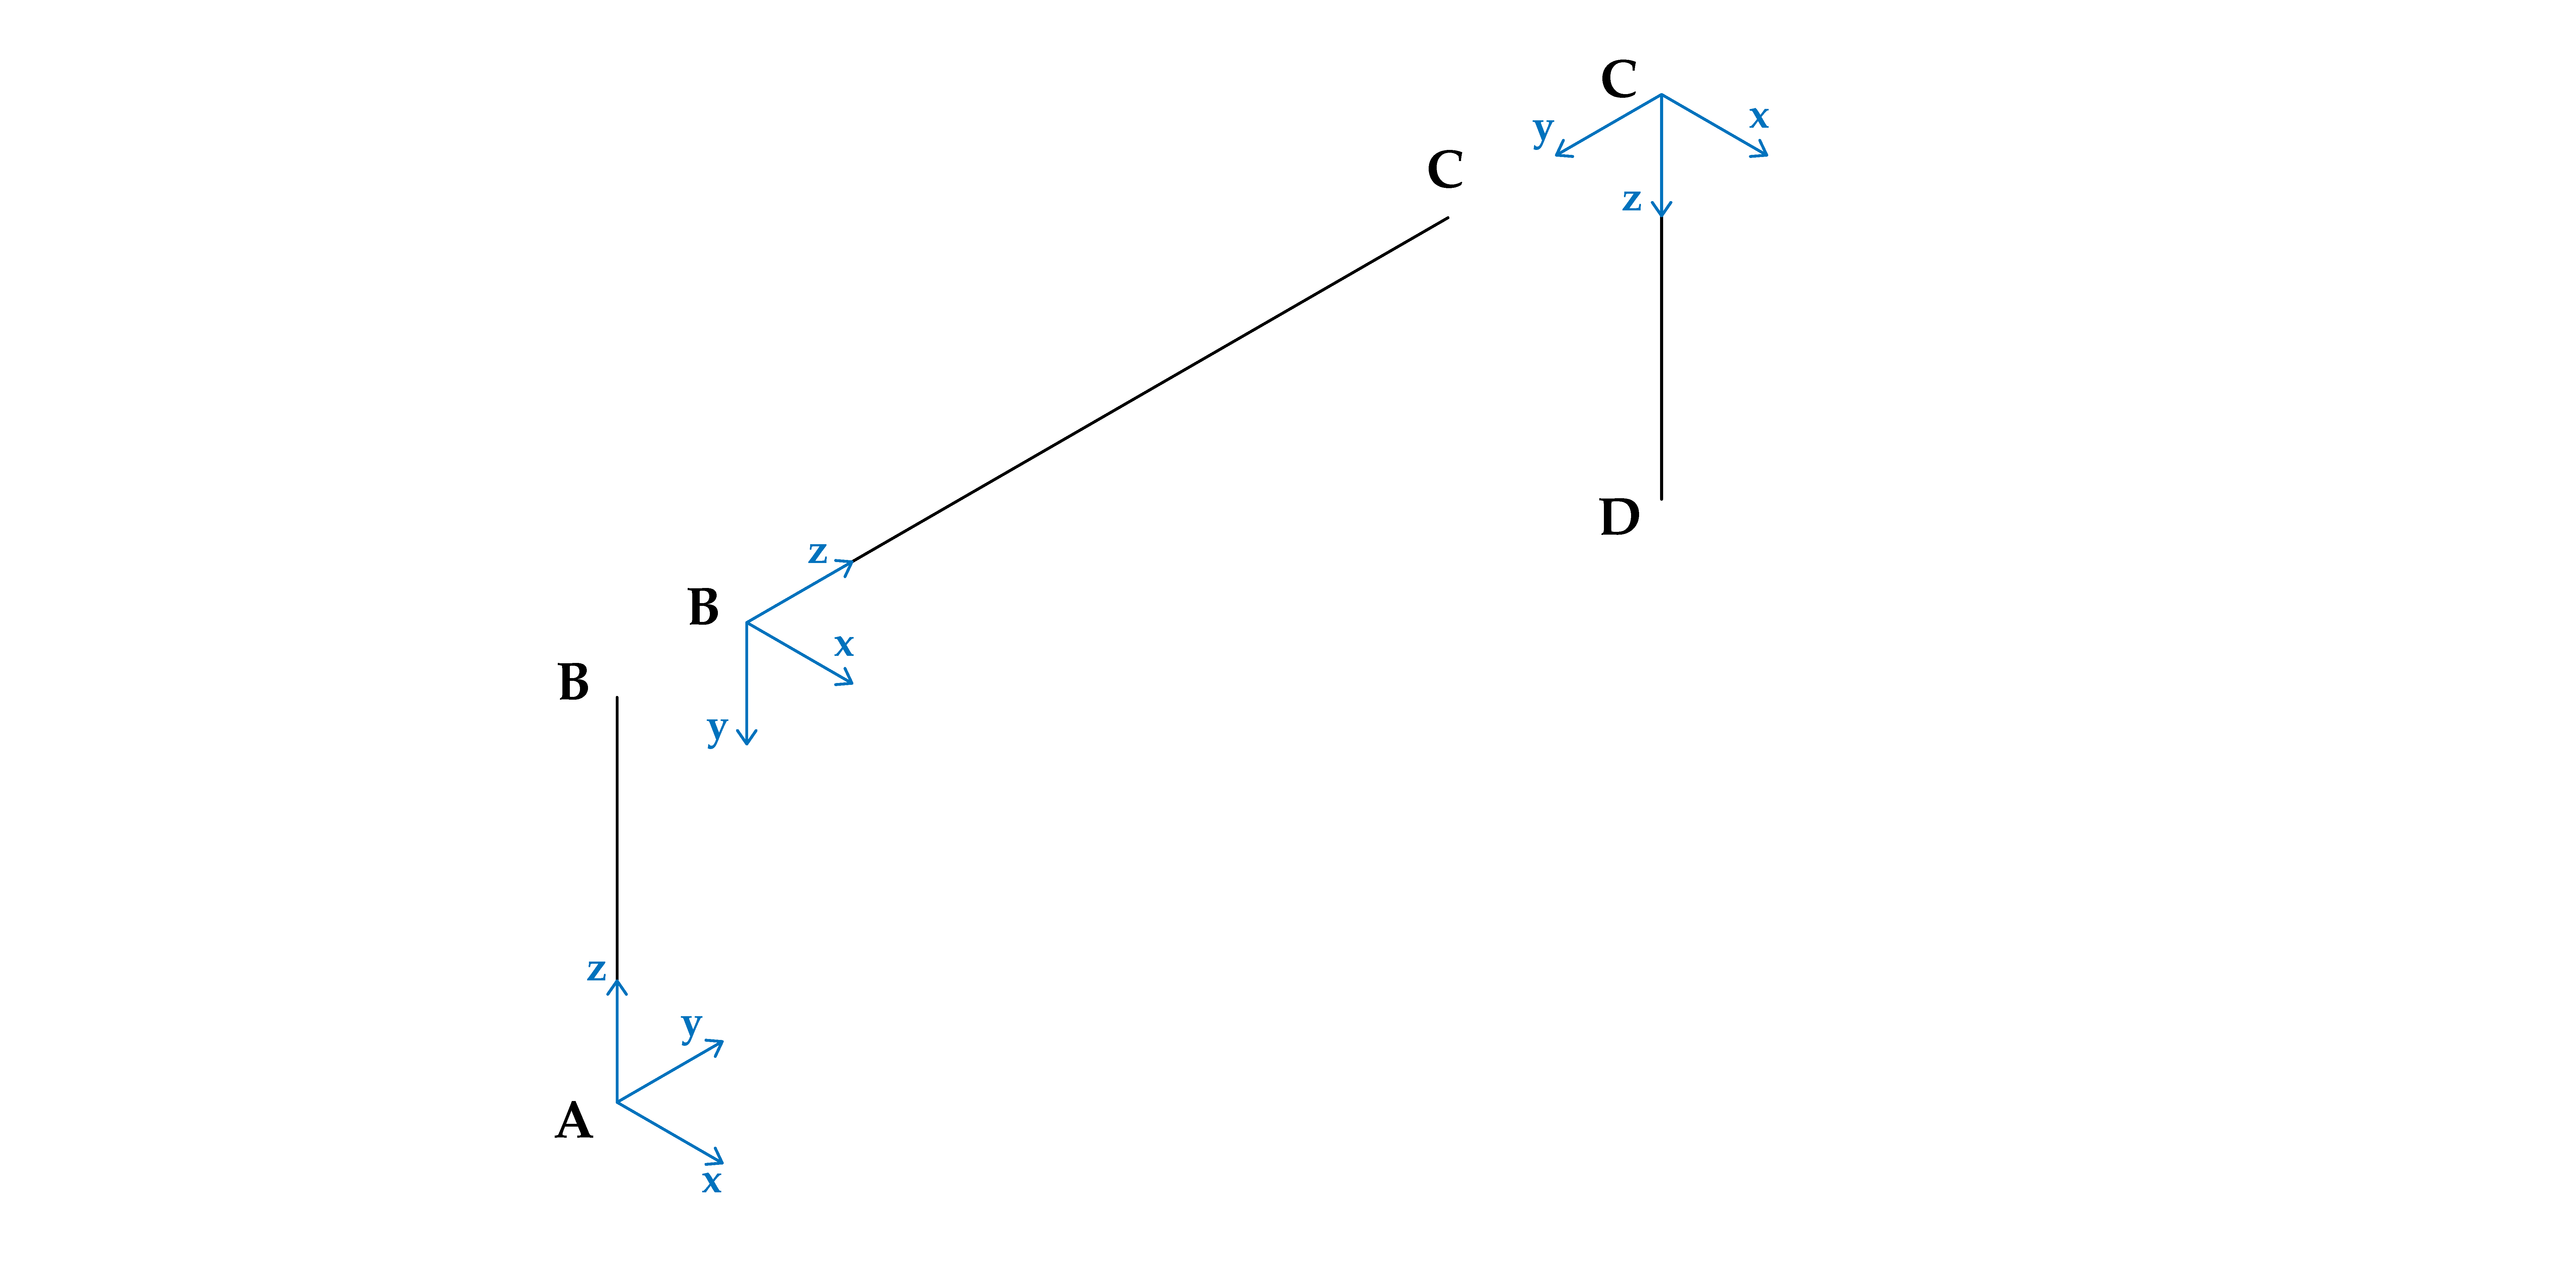
\includegraphics[width=15cm]{frames} \caption{}
		\end{subfigure}
		\caption{free body diagram (a) and reference frames (b) used for the description of the internal loads of the beam. In (a) the structure has been disassembled at the pivot point $C$ in order to describe the reaction forces transmitted.}
		\label{fig:fbd-frames}
	\end{figure}
	As simplification on both the geometry and the load we consider:
	\begin{itemize}
		\item on the elevated track the loads transferred by the working appendix are modelled as a pure vertical force $F$ (mainly related to the approximate weight of the turret that contains all equipment) and a torque $T$ that model's the one due to the plower; the eccentricities of both forces are in this case neglected and the application of application of both actions is placed at a distance $\zeta$ referred to the local coordinate $z$ of the elevated track, figure \ref{fig:fbd-frames}\textit{\textit{(b)}};
		
		\item the vertical supports are equally dimensioned and present a characteristic height $H = 700mm$; the elevated track connecting them has length $L = 3000mm$ as dictated by the customer requirements;
		
		\item figure \ref{fig:fbd-frames}\textit{(a)} shows the free body diagram of the structure and thus the set of external actions and reactions applied; figure \ref{fig:fbd-frames}\textit{(b)} reports instead the reference frames with respective origin with respect to which internal loads are calculated.
		
		The full joint in $B$ has not been described (as the connection preserves the continuity of the actions transmitted by the body), however the final design will imply the connection of two separate beams by means of a gusset.	
		
	\end{itemize}
	
	After having written the Newton-Euler equations of the two bodies making the whole structure, we observe that only 11 out of 14 reactions forces are independent; chosen the hyperstatic variables $X_1 = M_{Az},X_2 = M_{Dy}, X_3 = M_{Ax}$ to reduce the problem to an isostatic one, the parametric definitions of the reaction forces is
	\[ R_{Az} = \frac{F (L-\zeta) - X_3}{L} \qquad R_{Cz} = R_{Dz} =\frac{F\zeta + X_3}{L} \] \[ M_{Ay} = M_{Cy} = X_2 \qquad M_{Cz} = M_{Dz} = T-X_1 \]
	Non mentioned actions are identically zero. To solve the hyper-static problem the Castigliano's theorem has been used, computing the elastic energy $U_e$ of the structure neglecting shear loads:
	\[ U_e = \sum_{i=1}^3 \int_0 ^{l_i}  \left( \frac{N_i^2}{2EA_i} + \frac{M_{x,i}^2}{2 EI_{xx,i}} + \frac{M_{y,i}^2}{2 E I_{yy,i}} + \frac{M_{z,i}^2}{2G J_{t,i}}  \right)\, dz \]
	Assuming the generalized displacement related to the hyper-static variables is zero, solving the equations $\partial U_e / \partial X_i = 0$, the solution that we achieve is still depending on the geometrical parameters of the sections that are still unknown. To simplify the calculations we assumed $A_1 = 0$, giving the result
	\[ X_1 = T \qquad X_2 = 0 \qquad X_3 = F \frac{L-2\zeta}{2} \]
	
	
	In this preliminary design phase in order to over-estimate the loads the the frame should bear a force $F = 200 N$ is considered (modelling the weight of about $20kg$, related to all the carried equipment on the moving arm including batteries and filled water tank) and the nominal value of the torque $T = 0.8 N\cdot m$ as in the requirements specification.
	
	\paragraph{Choice of the standard beams} With the preliminary design model described, different solutions can be found looking from various vendors present in the marker. In particular for the project main reference has been made to the Parker IPS catalogue \cite{parker-ds} due to the high availability of accessories components, however similar product can be found by other vendors (as group we also evaluated 8020 \cite{8020-ds} and Tslots by Bonnel Aluminum \cite{tslot-ds}).
	
	Data-sheets presents information about the section area $A$ and second moments of area $I_{xx},I_{yy}$ respect the primary axes, however no information is given for the torsional rigidity $J_t$ and so the related component is in the calculation neglected. 
	
	\begin{table}[bt]
	\rule{\linewidth}{2pt}
	\caption{selected beams section chosen from the Parker IPS catalogue \cite{parker-ds} and related main properties (area, moments of inertia and weight per unit length).}
	\label{tab:beamchoice}
	\rule{\linewidth}{1pt} \vspace{0mm}	
	
	\begin{center}
		\begin{tabular}{p{3cm} | c c c c  |  l }
			& Area & \multicolumn{2}{c}{Moments of inertia} & Weight \\
			Usage & $A [cm^2]$ & $I_{xx} [cm^4]$ & $I_{yy} [cm^4]$ & $\rho [kg/m]$ & Product code \\ \hline
			track & 6.65 & 9.46 & 9.46 & 1.72 & \texttt{10-040} \\
			supports & 5.20 & 8.27 & 8.27 & 1.41 & \texttt{10-540} \\
		\end{tabular}
	\end{center}
	
	\vspace{3mm}
	\rule{\linewidth}{1pt}
	{\scriptsize
		\begin{multicols}{2}
		\begin{center}
			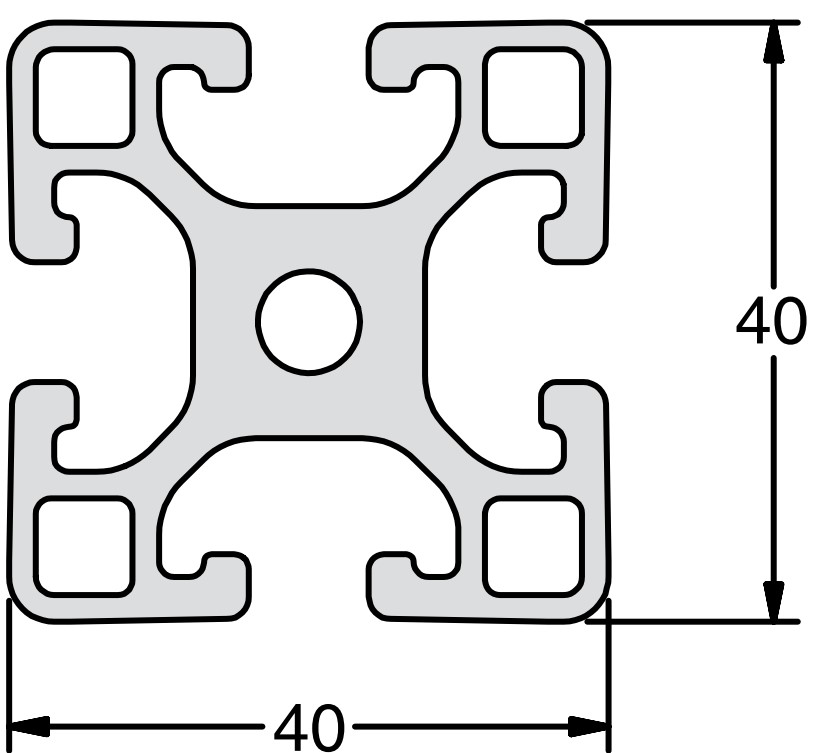
\includegraphics[height=2cm]{10-040}	\\		
			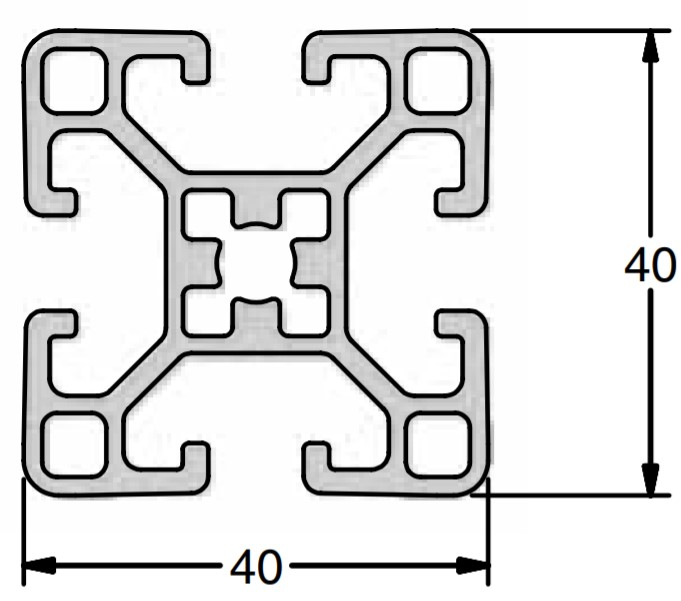
\includegraphics[height=2cm]{10-540}
		\end{center}
		\end{multicols}
		Sections for the track beam (on the left) and the supports (right).
	}	
	
	\rule{\linewidth}{2pt}
	
\end{table}
	
	After an iterative process, table \ref{tab:beamchoice} shows the sections drawing and associated geometric properties of the chosen components for both elevated track and supporting beams. This choice determines a safety factor $\phi = 3.8$ for the whole structure that's a safe value for us; it is true that we neglected both shear and torque loads, and in practical applications other external and unexpected actions might act on the frame, however it is also true that the geometric simplification $A_1 = 0$ in the solution of the hyperstatic problem heavily reduced the ability of the system to bear load (as we will see in the final static verification).
	
	As a side note, our design was forced to use the $40mm$ T-slot series (even if a $30mm$ profile would have let us achieve similar results with lower weights and costs) as it's the only one that disposes off-the-shelf linear roller system that can be easily mounted and used (choosing other profile series would have ended in custom solution that's undesired by the product design specifications).
	
	
	

	
	
	
	
	
	
	
	
	
	
	
	
	
	
	
	
	
	
	
	
	
	
	
	
	
	
	
	
	
	
	
	